\subsection{Scénario Cockburn}
\textbf{Cas d'utilisation:} Payer en liquide

\textbf{Acteur primaire:} Le Conducteur

\textbf{Pré-condition: } la borne affiche le montant
 

\textbf{Scénario primaire: } \\
    \textbf{1.} Le conducteur insère de l’argent liquide.\\
    \textbf{2.}  La borne enclenche la détection de fausse pièce. La borne valide les pièces.\\
    \textbf{3.} La borne analyse le montant . Le conducteur a donné le montant exact.\\
    \textbf{4.} La borne accepte le paiement.

\textbf{Variantes:}\\
    \textbf{2a.} La borne ne valide pas les pièces . La borne rend les pièces invalides.\\
    \textbf{3a.} La borne analyse le montant . Le conducteur donne un montant plus grand que celui de la borne. La borne rend la différence entre la somme introduite et le montant demandé.\\
    \textbf{3b.} La borne analyse le montant . Le conducteur donne un montant moins que celui de la borne. Se met en attente.\\
    \textbf{4a.} Le borne n’accepte pas le paiement. Appelle le technicien. \\
    \textbf{3a1.} La borne n’a plus de monnaie, la borne emet un signal pour avertir le technicien
\\
    
\newpage
\subsection{Diagramme d'activité}
\begin{figure}[h]
    \centering
    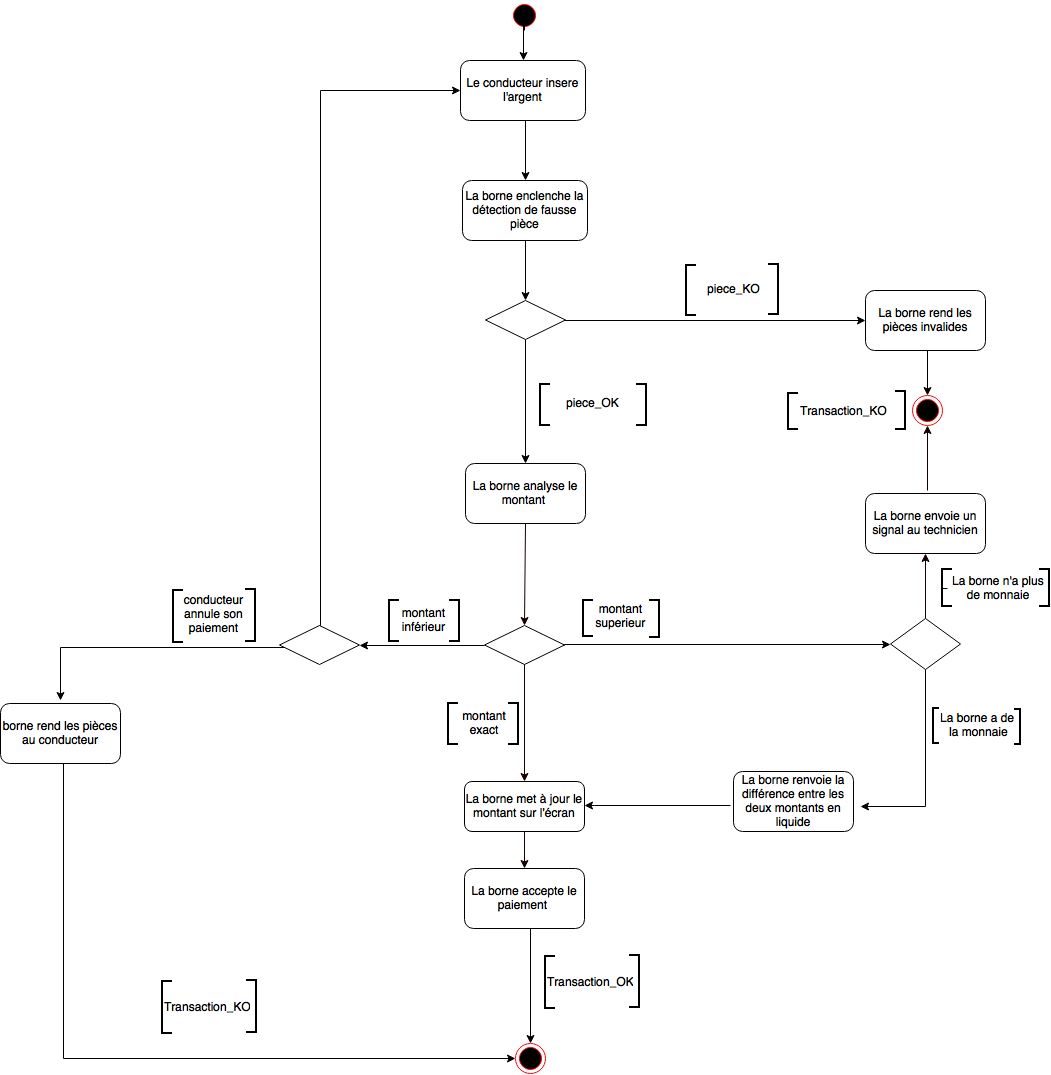
\includegraphics[scale=0.45]{02_Desenvolvimento/TD2/images/DAPayeLiquide.png}
    \caption{Diagramme d'activité: Payer en liquide}
\end{figure}
\newpage
\subsection{Collaboration}
\begin{figure}[h]
    \centering
    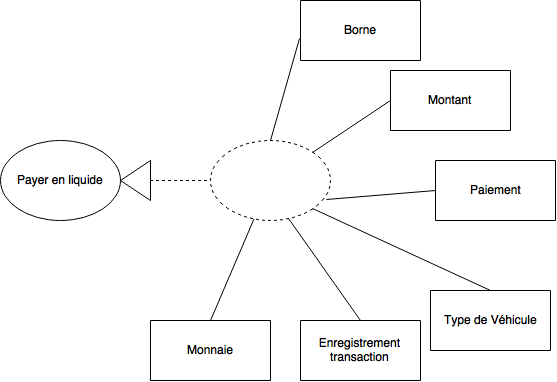
\includegraphics[scale=0.55]{02_Desenvolvimento/TD2/images/ColaLiquide.png}
    \caption{Collaboration: Payer en liquide}
\end{figure}